\documentclass[a4paper,11pt,ja=standard,xelatex]{bxjsreport}
% Embed static Japanese TrueType fonts for PDF viewer compatibility.
\setCJKmainfont[Path=C:/Windows/Fonts/,BoldFont=yumindb.ttf]{yumin.ttf}
\setCJKsansfont[Path=C:/Windows/Fonts/,BoldFont=meiryob.ttc]{meiryo.ttc}
\setCJKmonofont[Path=C:/Windows/Fonts/,BoldFont=meiryob.ttc]{meiryo.ttc}
\usepackage{amsmath,amssymb,booktabs,longtable,array,multirow}
\usepackage{graphicx,float,caption,subcaption,tikz,pgfplots,xcolor,hyperref,url,enumitem}
\usepgfplotslibrary{groupplots}\pgfplotsset{compat=1.18}
\hypersetup{colorlinks=true,linkcolor=blue,citecolor=blue,urlcolor=blue}
\setlength{\parskip}{0.25em}\setlength{\parindent}{1em}\renewcommand{\arraystretch}{1.16}
\title{UAV農作物画像におけるDepth Anything V2 Smallの\\Metric Depth適応と局所深度構造の評価}
\author{著者名・所属：提出前に記入}\date{2026年10月14日}
\begin{document}\maketitle\pagenumbering{roman}
\chapter*{要旨}\addcontentsline{toc}{chapter}{要旨}
農作物の生育状態を広域・反復的に把握する手段としてUAV画像と深度推定を組み合わせた計測が期待される。しかし単眼モデルのカメラ座標系深度は、地表から植物頂部までの垂直距離である草丈とは異なる。本研究ではDepth Anything V2 SmallをUAV3DCropのCorn、Oat、Wheat、Soybean画像へ適応した第1〜3回実験を再整理し、絶対深度誤差と局所深度構造を別々に評価した。学習384組（Day019、028、040）、検証128組（Day047）を用い、独立test319組および過去52組は未使用とした。モデルAはRelative Small由来backboneに新規Metric headを設け1 epoch学習、Bは未学習Metric Outdoor Small、Cは同モデルを1 epoch追加学習、Dは元のMetric Outdoor Smallから独立した20 epoch計画runを開始しepoch 5まで学習した。
共通validationのRMSEはBの14.5340 mからCの1.7490 m、D epoch 5の1.0094 mへ低下した。D epoch 5はMAE 0.7373 m、AbsRel 0.03694、Pearson 0.9919、14 px局所差MAE 0.06148 mであった。一方、GT差20 cm以上の標本では振幅比0.3304、符号一致率81.02\%で、大きな変化の過小推定が残った。第2回分析ではAの局所誤差増加が画像端128 px以内に集中し、同帯は標本ペア10.90\%でA−B局所MAE増分の82.52\%を占めた。局所変化ゼロの基準が総局所MAEに有利となり得ることも確認した。結果はカメラZ-depthに対するもので、垂直草丈や稲高を実証しない。独立test、複数seed、稲高GTは今後の課題である。
\noindent\textbf{キーワード：}単眼深度推定，Metric Depth，UAV，局所深度差，草丈
\tableofcontents\listoffigures\listoftables
\clearpage\pagenumbering{arabic}
\chapter{序論}
\section{背景}
作物の草丈は生育段階、栄養状態、倒伏リスク、収量形成などを把握する重要な表現型である。定規等による地上計測は直接的である一方、多数個体を反復して測るには労力がかかる。UAV画像は広域を短時間で取得でき、画像処理や写真測量と組み合わせた高スループットな表現型計測を可能にする。UAV画像・LiDARを用いた作物高推定は、作物、撮影時期、地面モデル、視線・スキャン角度に依存することが報告されている\cite{cropheight,uav3dcrop}。
単眼深度推定は一枚のRGB画像から各画素の奥行きを推定するため、追加深度センサを必要としない。視覚基盤モデルの特徴を下流タスクへ転移することで、単眼深度推定にも適応が可能となった\cite{dinov2,dav2}。ただし単眼画像から尺度を一意に定めることは原理的に困難であり、学習分布や幾何的手がかりに依存する\cite{eigen2014}。屋外一般シーンで学習されたMetric Depthモデルは、葉群、細い茎、列状植生、露出土壌、遮蔽が混在する農作物画像で尺度誤差や局所平滑化を生じ得る。
\section{目的と貢献}
本研究はDepth Anything V2 SmallのMetric Depth出力を農作物UAV画像に適応し、絶対深度精度と局所深度変化がどのように推移するかを既実施3実験から検討する。貢献は、(1) Relative由来Metric head、未学習Metric Outdoor、1 epoch追加学習、独立した5 epoch runを共通validationの定義に注意して統合すること、(2)局所差分の振幅・符号・GT差分階級・画像端の詳細分析から全体局所MAEの限界を示すこと、(3) epoch 1--5曲線から絶対値と局所形状の非同値性、再現性、未検証事項を記録することである。本稿は実施済み実験の中間報告であり、稲の垂直草丈または独立test性能を報告するものではない。\chapter{関連研究と理論}
\section{単眼深度推定}
単眼画像$I$から深度場$D$を求める問題は画素ごとの回帰$D=f_\theta(I)$として表される。単眼投影では物体の大きさと距離の組合せが同じ画像を生じ得るため、尺度は画像内容のみから常に一意ではない。Relative Depthは主に前後関係や相対構造を表し、Metric Depthはメートル等の実尺度を出力する。Relative checkpointをMetric推定へ転用するには、尺度を学ぶheadとMetric教師が必要である。
\section{Depth Anything V2、ViT、DPT}
Depth Anything V2は大規模な合成深度教師と実画像擬似ラベルを組み合わせた単眼深度モデルであり、複数規模のモデルと屋内・屋外Metric checkpointが公開されている\cite{dav2}。SmallはDINOv2 ViT-S/14系encoderから得る中間特徴を用いる\cite{dinov2}。Vision Transformer（ViT）は画像をpatch token列へ写像し、Self-Attentionにより文脈特徴を学習する\cite{vit2021}。Dense Prediction Transformer（DPT）は異なるTransformer層の特徴を解像度別のマップへ射影し、融合ブロックで段階的に統合して密な画素予測を行う\cite{dpt2021}。したがって出力は単一patchの分類ではなく、encoder特徴とdecoder再構成の組合せである。
Metric Depth実装はhead出力をsigmoidで$[0,1]$へ写像し、モデル上限$M$でスケールする。本研究ではGTマスク上限とforward係数を別パラメータにした。$M$は予測可能深度範囲、$G$はloss・評価で採用するGT画素範囲である。
\section{転移学習とSiLog}
事前学習特徴を新しい分布へ適応する転移学習として、本研究はRelative backboneからMetric headを学ぶAと、Metric Outdoor全体を追加更新するC/Dを比較した。尺度不変対数損失（SiLog）は$g_i=\log\hat d_i-\log d_i$に基づき、対数誤差の二乗平均から共通対数尺度偏差成分を控除する\cite{eigen2014}。
\[
L_{\mathrm{SiLog}}=\sqrt{\frac1N\sum_{i=1}^N g_i^2-\lambda\left(\frac1N\sum_{i=1}^N g_i\right)^2},\quad \lambda=0.5.
\]
この構成は相対的な誤差と尺度バイアスを同時に扱うが、14 px差分を直接最小化する損失ではない。本稿の学習ではSiLogを変更していない。
\section{写真測量深度と植物高}
UAV3DCropは反復・複数視点UAV画像と写真測量由来幾何情報を含むベンチマークである\cite{uav3dcrop}。本研究のGTはカメラ座標系の光軸方向Z-depthであり、世界座標系の鉛直軸高さではない。草丈の計算には植物頂部と地面の対応、カメラ姿勢・内部標定、座標変換が必要である。よって本研究の深度差分は植物垂直高差の教師ではない。
\chapter{データセットと前処理}
\section{対象データと分割}
UAV3DCropのCorn、Oat、Wheat、Soybeanから、RGBと対応深度GTの512組、計1024ファイルを使用した。記録された転送量は7,850,330,776 byteである。データは第1回実験時にGoogle Driveへ保存され、第2・3回で再利用された。本報告書作成時にデータは再取得・再監査していない。
\begin{table}[H]\centering\caption{実験で使用した分割}\label{tab:split}
\begin{tabular}{llll}\toprule 用途&撮影日&組数&使用\\\midrule
学習&Day019, Day028, Day040&384&学習\\
検証&Day047&128&各runのvalidation\\
独立test&未取得&319&未使用\\
過去評価&過去の52組&52&モデル選択に未使用\\\bottomrule\end{tabular}
\end{table}
撮影日単位で分割し、同じ日の類似画像がtrain/validation間へ混在するリスクを抑えた。ただし、未知日・未知圃場への汎化を保証するものではない。独立testはモデル選択完了まで未使用に保留された。
\section{GTと前処理}
RGBと深度は元解像度3956$\times$5280 pixelで管理された。train GT最大値は62.15625 m、99.9 percentileは52.90625 mである。train最大値を包含する教師・評価上限として$G=65$ mを設定した。これはvalidation/testによる選択ではない。無効値は0で、GTが有限かつ正かつ65 m以下の画素だけを有効とした。
学習は518$\times$518 cropを入力とする。検証はアスペクト比を保持して短辺518、長辺約686 pixelへresizeし、予測を元サイズへ復元して評価した。元短辺3956 pixelから518への倍率は約7.64であり、元画像14 pixel間隔はモデル入力上約1.83 pixelとなる。ViTの14 pixel patchを目安とすると元画像上約107 pixelに対応する。DPTは多解像度特徴を融合するものの、縮小で葉・茎・株境界の情報が弱まる可能性がある。
\section{深度と草丈の違い}
GT Zはカメラ光軸方向に沿う距離である。Obliqueでは地面平面も画像内で奥行き変化をもつ。カメラ俯角のある鉛直植物は、見かけのZ変化が高さと単純比例しない。草丈評価には共通世界座標で地面と頂部を対応づけ、鉛直成分を計算する必要がある。したがって20 cmのZ差は垂直草丈20 cmを意味しない。\chapter{学習手法}
\section{比較モデル}
全モデルはDepth Anything V2 Small系ViT-S/14 encoderとDPT型密予測headを基礎とする\cite{dav2,dpt2021}。
\begin{description}[leftmargin=2.6em,style=nextline]
\item[モデルA] Relative Small backboneを転用し、Metric neck/headを新規初期化して1 epoch学習。model output capは65 m。
\item[モデルB] 追加学習前のMetric Outdoor Small。output cap 80 m。
\item[モデルC] Metric Outdoor Small重みから1 epoch追加学習した第2回モデル。cap 80 m。
\item[モデルD] 元の未追加学習Metric Outdoor Smallから独立runとして開始した第3回モデル。20 epoch計画でepoch 5まで実行。Cのcheckpointから継続していない。cap 80 m。
\end{description}
Aは初期化方式だけでなく出力上限もB--Dと異なるため、上限の寄与を単独で分離した比較ではない。全モデルのGT maskは$G=65$ mで共通とし、B--D予測を65 mに再スケールまたはclipしていない。
\section{forwardと有効GT}
head未正規化出力を$z_\theta(I)$とすると
\[
\hat d(I)=M\sigma(z_\theta(I)),\qquad
\mathcal{V}=\{i:d_i^*>0,\ d_i^*\le G,\ d_i^*\text{ finite}\},\quad G=65\ {\rm m}.
\]
$M$はforward出力係数、$G$はloss・評価に使うGT上限である。これらを同じ設定値にすると、出力範囲を65 mに変えただけで同一weightの予測が80 m時の65/80倍へ変化する。第2回の実画像probeでこの現象を確認したため、コードで分離した。
\section{学習条件とscheduler}
基準runはSiLog、AdamW\cite{adamw}、seed 42、batch 1、gradient accumulation 4、AMPを用いた。encoder LR $5\times10^{-6}$、neck/head LR $5\times10^{-5}$である。384画像・batch 1は1 epoch 96 planned optimizer updates、20 epoch計画は1920 updateとなる。DのPolynomialLR総期間は1920 updateのまま維持された。AMP skip時はoptimizer update・schedulerを進めない。epoch 1にskipが1回あり、epoch 5時点schedulerは成功update 479回に対応する。Cの1 epoch runとDでは総scheduler期間と履歴が異なり、両者の差をepoch数だけの因果効果とみなさない。
\section{checkpoint管理}
各epoch境界でmodel、optimizer、scheduler、GradScaler、乱数状態を含むcheckpointとmetadataを保存した。第3回はepoch 0--5 complete checkpoint、run metadata、status、epoch metrics CSV/JSON、training log、sync receiptをDriveへ保存した。今回の論文作成中にcheckpointの再読み込みや再推論はしていない。Dは5/20 epochで安全停止中である。
\chapter{評価方法}
\section{絶対深度指標}
有効画素数を$N$、予測深度を$\hat d_i$、GTを$d_i$とする。平均絶対誤差、二乗平均平方根誤差、絶対相対誤差は
\[
\mathrm{MAE}=\frac1N\sum_i|\hat d_i-d_i|,\quad
\mathrm{RMSE}=\sqrt{\frac1N\sum_i(\hat d_i-d_i)^2},\quad
\mathrm{AbsRel}=\frac1N\sum_i\frac{|\hat d_i-d_i|}{d_i}
\]
である。RMSEは大誤差を二乗で重みづけ、AbsRelはGT距離に対する誤差比を表す。Pearson相関$r$は有効画素上の予測とGTの線形相関であり、尺度バイアス自体を測らないため絶対誤差と併記した。深度MAE等は元解像度へ復元後の全validation画素集計である。
\section{局所深度差指標}
元画像座標で水平方向または垂直方向に14 pixel離れた有効画素対$(i,j)$について、
\[
\Delta d_{ij}=d_j-d_i,\quad \Delta\hat d_{ij}=\hat d_j-\hat d_i,\quad
E_\Delta=\frac1P\sum_{(i,j)}|\Delta\hat d_{ij}-\Delta d_{ij}|
\]
を14 px局所深度差MAEとした。ペア両端がGT有効mask内にあるものを採用する。これは画素深度の絶対誤差ではなく差分誤差である。
GT絶対差分が20 cm以上の固定標本に対して、差分振幅比を
\[
R_{\mathrm{amp}}=\frac{\operatorname{mean}|\Delta\hat d|}{\operatorname{mean}|\Delta d|}
\]
と定義した。比が1未満なら平均振幅を過小推定する。符号一致率はGT差分非ゼロのペアで$\mathrm{sign}(\Delta\hat d)=\mathrm{sign}(\Delta d)$となる割合で、予測0は不一致とする。差分相関は$\Delta d,\Delta\hat d$のPearson相関、回帰傾きは切片を含む最小二乗回帰$\Delta\hat d=a+b\Delta d+\epsilon$の$b$である。回帰で予測を補正していない。
\section{全ペア・固定標本・基準値}
絶対深度と14 px局所MAEは全有効画素・全有効ペアで計算した。GT差分階級、符号、振幅・相関・回帰、画像端帯は固定座標標本による詳細集計である。第2回の14 px固定標本は25,552,938 pairと報告され、候補座標はモデル共通、seed規則が保存された。標本値を全ペア値と混同しない。第3回CSVはfull-pair列とsampled列を分けるが、固定標本数が報告資料で照合できない項目は本稿で25,552,938と仮定しない。
局所変化を常に0とする基準では$\Delta\hat d=0$となり、局所MAEはGTペアの平均絶対差分である。このゼロ差分基準は絶対深度MAE/RMSEを定義しない。第2回の全14 pxペア値は0.06421224 mであった。GT差分が小さいペアが多いと平坦予測が総合局所MAEで有利になり得る。
\section{境界と統計単位}
画像端からの最短距離で0--128 px、128--512 px、512 px以上に分類した。主指標は全画面評価のままであり、端除外値は診断である。validation 128画像内の画素・ペアは空間自己相関をもつ。数十億画素を独立標本として信頼区間や有意差検定を行っていない。画像単位の再標本化に必要な統一画像単位集計を根拠一式から確認できないため、信頼区間・有意差を報告しない。\chapter{実験結果}
\section{モデルA--Dの主比較}
表\ref{tab:maincompare}は共通validationの確定済み結果である。A/Bは第1回、Cは第2回、Dは第3回epoch 5である。絶対指標は有効画素、local14は全有効ペアで集計した。
\begin{table}[H]\centering\scriptsize
\caption{共通validationにおける主要モデル比較}\label{tab:maincompare}
\begin{tabular}{lrrrrrr}\toprule
モデル&epoch&MAE m&RMSE m&AbsRel&Pearson $r$&local14 MAE m\\\midrule
A Relative由来Metric&1&2.4897&3.9063&.12120&.8712&.10545\\
B 未学習Metric Outdoor&0&13.2730&14.5340&.65896&.7848&.06561\\
C Metric Outdoor追加学習&1&1.1324&1.7490&.05208&.9773&.06800\\
D Metric Outdoor独立run&5&.7373&1.0094&.03694&.9919&.06148\\\bottomrule
\end{tabular}\end{table}
Bの局所差MAEがCより僅かに低いことだけで形状復元が優れるとは言えない。第2回ゼロ差分基準0.06421 mに対しBは0.06561 m、Cは0.06800 mである。Dは全ペアlocal14が0.06148 mとなり、この基準を下回った。
\section{第3回epoch別推移}
表\ref{tab:epochs}はDriveの第3回epoch CSVと報告表の値である。GT差20 cm以上の局所MAE、振幅比、符号、画像端・内部は固定標本、local14は全有効ペア指標である。
\begin{table}[H]\centering\scriptsize
\caption{モデルDのepoch別validation結果}\label{tab:epochs}
\begin{tabular}{rrrrrrrrrrr}\toprule
Ep.&SiLog&MAE&RMSE&AbsRel&$r$&local14&GT$\geq$20cm MAE&振幅比&符号&秒\\\midrule
1&.10622&1.0791&1.6299&.05088&.9805&.06537&.35276&.3046&78.28\%&1085.5\\
2&.05288&1.7002&1.9953&.08907&.9884&.06339&.34543&.3263&80.24\%&1044.1\\
3&.03596&1.0492&1.3334&.05726&.9894&.06299&.34708&.3228&80.82\%&1097.8\\
4&.03025&.7744&1.0562&.03913&.9901&.06237&.34495&.3428&80.52\%&1024.4\\
5&.02794&.7373&1.0094&.03694&.9919&.06148&.34090&.3304&81.02\%&1020.9\\\bottomrule
\end{tabular}\end{table}
\noindent\small MAE/RMSE/GT局所MAE/local14はm、振幅比・損失は無次元、Pearsonは$r$である。各epochのVRAM peakはallocated 0.877 GiB、reserved 1.248 GiB。AMP skipはepoch 1が1回、epoch 2--5は0回。\normalsize
\begin{figure}[H]\centering
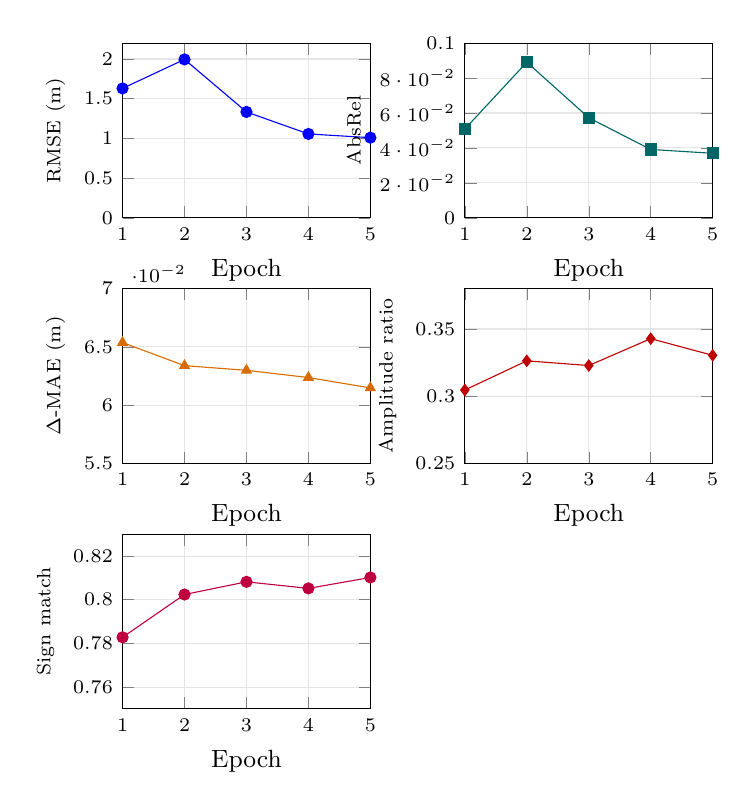
\begin{tikzpicture}
\begin{groupplot}[group style={group size=2 by 3,vertical sep=.9cm,horizontal sep=1.2cm},
width=.39\textwidth,height=3.8cm,grid=major,grid style={gray!20},
xlabel={Epoch},xmin=1,xmax=5,xtick={1,2,3,4,5},tick label style={font=\scriptsize},label style={font=\small},ylabel style={font=\scriptsize}]
\nextgroupplot[ylabel={RMSE (m)},ymin=0,ymax=2.2]\addplot[blue,mark=*] coordinates{(1,1.6299)(2,1.9953)(3,1.3334)(4,1.0562)(5,1.0094)};
\nextgroupplot[ylabel={AbsRel},ymin=0,ymax=.10]\addplot[teal!80!black,mark=square*] coordinates{(1,.05088)(2,.08907)(3,.05726)(4,.03913)(5,.03694)};
\nextgroupplot[ylabel={$\Delta$-MAE (m)},ymin=.055,ymax=.070]\addplot[orange!85!black,mark=triangle*] coordinates{(1,.06537)(2,.06339)(3,.06299)(4,.06237)(5,.06148)};
\nextgroupplot[ylabel={Amplitude ratio},ymin=.25,ymax=.38]\addplot[red!75!black,mark=diamond*] coordinates{(1,.3046)(2,.3263)(3,.3228)(4,.3428)(5,.3304)};
\nextgroupplot[ylabel={Sign match},ymin=.75,ymax=.83,ytick={.76,.78,.80,.82}]\addplot[purple,mark=*] coordinates{(1,.7828)(2,.8024)(3,.8082)(4,.8052)(5,.8102)};
\end{groupplot}\end{tikzpicture}
\caption{第3回モデルDのepoch曲線。既存epoch CSVの数値から再描画した。RMSE/AbsRelは全validation画素、$\Delta$-MAEは全有効14 pxペア、振幅比・符号一致はGT差20 cm以上の固定標本である。縦軸範囲は指標ごとに異なる。}\label{fig:curves}\end{figure}

epoch 2ではRMSEが1.6299 mから1.9953 m、MAEが1.0791 mから1.7002 m、AbsRelが0.05088から0.08907へ一時悪化した。一方local14は0.06537 mから0.06339 mへ改善し、振幅比・符号一致も上昇した。epoch 3--5で絶対誤差は低下し、epoch 5に最小値となった。複数指標は単調に同時改善していない。
\section{GT差20 cm以上の局所構造}
第2回モデルCでは、GT差20 cm以上の標本平均絶対差分0.44370 m、予測平均振幅約0.1453 m、振幅比0.327であった。該当区間局所MAEは0.35423 m、符号一致77.95\%であり、86.72\%のペアで振幅を過小推定した。第3回Dではepoch 1から5へ振幅比0.3046から0.3304、区間MAE0.35276 mから0.34090 m、符号一致78.28\%から81.02\%へ変化した。改善はあるが単調ではない。CとDの振幅比の差は小さいが、標本抽出条件を厳密に突合できないため対応のある差分比較とは解釈しない。
\begin{figure}[H]\centering\begin{tikzpicture}
\begin{axis}[width=.82\textwidth,height=6cm,ybar,bar width=12pt,
symbolic x coords={small,mid1,mid2,large},xtick=data,xticklabels={0--5 cm,5--10 cm,10--20 cm,$\geq$20 cm},
ylabel={Local delta MAE (m)},ymin=0,ymax=.48,
legend style={at={(.5,1.06)},anchor=south,legend columns=2,font=\scriptsize},grid=major,grid style={gray!20}]
\addplot[fill=gray!60] coordinates{(small,.01617)(mid1,.07304)(mid2,.14112)(large,.44370)};
\addplot[fill=blue!70] coordinates{(small,.07480)(mid1,.09063)(mid2,.12255)(large,.41357)};
\addplot[fill=orange!80] coordinates{(small,.02266)(mid1,.06963)(mid2,.12858)(large,.41684)};
\addplot[fill=green!65!black] coordinates{(small,.03451)(mid1,.07031)(mid2,.10600)(large,.35423)};
\legend{Zero baseline,A Relative由来,B 未学習,C 1 epoch}
\end{axis}\end{tikzpicture}
\caption{第2回のGT差分階級ごとの局所深度差MAE。各値は報告済み固定標本。小差分の多数ペアと20 cm以上のペアでモデル順位が異なる。}\label{fig:bins}\end{figure}

第2回GT差分階級標本の72.96\%は0--5 cmであった。同階級の局所MAEはゼロ基準0.01617 mに対しA 0.07480 m、B 0.02266 m、C 0.03451 mである。20 cm以上ではゼロ基準0.44370 m、A 0.41357 m、B 0.41684 m、C 0.35423 mとなり、Cは大きい差分を小さくする誤差を相対的に減らした。
\section{画像端と画像内部}
\begin{figure}[H]\centering\begin{tikzpicture}
\begin{axis}[width=.84\textwidth,height=6.2cm,ybar,bar width=15pt,
symbolic x coords={edge,transition,interior},xtick=data,
xticklabels={0--128 px,128--512 px,$\geq512$ px},
ylabel={14 px local delta MAE (m)},ymin=0,ymax=.43,
legend style={at={(.5,1.06)},anchor=south,legend columns=2,font=\scriptsize},grid=major,grid style={gray!20}]
\addplot[fill=blue!70] coordinates{(edge,.38929)(transition,.09682)(interior,.05814)};
\addplot[fill=orange!80] coordinates{(edge,.08717)(transition,.07033)(interior,.05945)};
\addplot[fill=green!65!black] coordinates{(edge,.09189)(transition,.07112)(interior,.06220)};
\addplot[fill=gray!60] coordinates{(edge,.07866)(transition,.06898)(interior,.05934)};
\legend{A Relative由来,B 未学習,C 1 epoch,ゼロ差分}
\end{axis}\end{tikzpicture}
\caption{第2回固定標本における画像端距離別14 px局所差MAE。端0--128 px帯はペアの10.90\%だが、Aの誤差が突出する。}\label{fig:edge}\end{figure}

第2回標本の画像端0--128 pxではA局所MAE 0.38929 m、B 0.08717 m、C 0.09189 mであった。この帯のペア割合は10.90\%だが、A−Bの総局所MAE増分の82.52\%を占めた。端から512 px以上の内部ではA 0.05814 m、B 0.05945 m、C 0.06220 mとなり順位が逆転する。D epoch 5は端0--128 pxのsampled local MAE 0.08095 m、内部512 px以上0.05678 mである。GT差20 cm以上のDでは端MAE0.36135 m、振幅比0.4951、符号84.40\%、内部MAE0.35727 m、比0.2028、符号77.67\%である。標本結果であり因果効果ではない。
\section{作物・撮影方向別}
\begin{table}[H]\centering\small
\caption{モデルD epoch 5の作物別結果}\label{tab:crop}
\begin{tabular}{lrrrr}\toprule 作物&MAE m&RMSE m&AbsRel&local14 MAE m\\\midrule
Corn&1.00694&1.30455&.04711&.08305\\
Oat&.89419&1.13390&.04414&.06255\\
Soybean&.60541&.86185&.03249&.04892\\
Wheat&.44293&.58861&.02403&.05142\\\bottomrule\end{tabular}\end{table}
\begin{table}[H]\centering\small
\caption{モデルD epoch 5の撮影方向別結果}\label{tab:view}
\begin{tabular}{lrrrrr}\toprule 方向&MAE m&RMSE m&AbsRel&Pearson $r$&local14 MAE m\\\midrule
Nadir&.57857&.75396&.03704&.79186&.03649\\
Oblique&.89654&1.21291&.03684&.99173&.08657\\\bottomrule\end{tabular}\end{table}
ObliqueはNadirよりMAE、RMSE、局所14 MAEが大きい。Pearsonの方向差は深度分布レンジや画像混合集計の影響を受けるため、単独で難易度を決めない。作物・方向・深度範囲が均衡化された要因実験ではないため、差を作物固有の原因へ帰属させない。
\section{checkpoint選択}
第3回報告書ではvalidation RMSE最良はepoch 5（1.0094 m）、GT差20 cm以上の標本局所MAE最良もepoch 5（0.34090 m）である。ただし振幅比はepoch 4の0.3428が最高、符号一致と全14 px MAEはepoch 5が最良である。「局所形状最良」は単一の報告済み選択基準に限った呼称であり、総合最良を意味しない。独立testは未使用である。
\begin{figure}[H]\centering
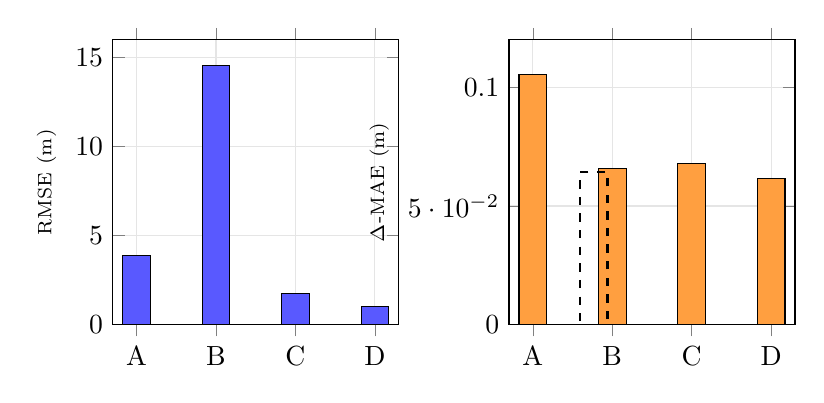
\begin{tikzpicture}\begin{groupplot}[group style={group size=2 by 1,horizontal sep=1.4cm},width=.43\textwidth,height=5.2cm,ybar=12pt,grid=major,grid style={gray!20},symbolic x coords={A,B,C,D},xtick=data,ylabel style={font=\scriptsize}]
\nextgroupplot[ylabel={RMSE (m)},ymin=0,ymax=16]\addplot[fill=blue!65] coordinates{(A,3.9063)(B,14.5340)(C,1.7490)(D,1.0094)};
\nextgroupplot[ylabel={$\Delta$-MAE (m)},ymin=0,ymax=.12]\addplot[fill=orange!75] coordinates{(A,.10545)(B,.06561)(C,.06800)(D,.06148)};
\addplot[black,dashed,thick,forget plot] coordinates{(A,.064212)(D,.064212)};
\end{groupplot}\end{tikzpicture}
\caption{モデルA--Dのvalidation比較。左は全有効画素RMSE、右は全有効14 pxペア局所MAE。破線は第2回ゼロ差分基準0.06421 m。}\label{fig:compare}\end{figure}




\chapter{考察}
\section{Metric Outdoor事前学習からの適応}
BからCのMAEは13.2730 mから1.1324 m、RMSEは14.5340 mから1.7490 m、AbsRelは0.65896から0.05208へ低下した。BとCはMetric Outdoor由来で出力cap80 mを維持し、同じDay047 validationと65 m以下のGT maskで比較されている。このvalidationにおいて、1 epochの農作物データ適応後に大きな絶対深度改善が観測されたと結論できる。Dは同じ未学習Metric Outdoor初期値から独立に始め、epoch 5のRMSEは1.0094 mであった。ただしCとDはscheduler総期間とrun履歴が異なるため、この差を純粋なepoch数の効果とは断定しない。
\section{絶対深度と局所形状の非同値性}
SiLogは対数深度残差を通して深度場を最適化するが、14 px差分誤差を直接最小化する目的ではない。絶対値や低周波構造が合っても、葉縁等の高周波形状は平滑化され得る。Dの全14 px MAEはepoch 1--5で0.06537から0.06148 mへ改善した一方、GT差20 cm以上の振幅比は0.3046--0.3428で変動し、epoch 5では0.3304であった。absolute depth改善と局所振幅改善は同じ速度・方向ではない。
epoch 2はMAE/RMSE/AbsRelがepoch 1より悪化したが、Pearson、局所14 MAE、振幅比、符号一致は改善した。重み更新、validation分布、最適化状態のどれが原因か保存ログからは特定できない。短いrunにおける非単調推移として扱う。
\section{ゼロ差分基準の含意}
ゼロ差分基準0.06421 mは、GT差分が平坦なペアの多い14 px集計で、常に変化なしとする予測が小さいlocal MAEを得る場合を示す。Bの振幅比は0.3083で、全局所MAE0.06561 mもゼロ基準に近い。これはBの形状が忠実という証拠ではなく、評価平均が振幅縮小に利点を与えることと整合する。GT差0--5 cmが標本の72.96\%を占める一方、20 cm以上は7.48\%である。GT階級、振幅、符号、相関、複数間隔を併記しなければ大きい構造の復元状態を見落とす。
CはGT差20 cm以上でBよりMAEが小さく、符号一致も高いが、振幅比0.327は過小推定を示す。D epoch 5も0.3304であり、課題は残る。第2回と第3回の標本抽出件数・抽出署名の完全な一致は根拠資料から照合できず、CとDの差を対応のある効果量として解釈しない。
\section{Relative由来Aの画像端偽勾配}
第2回では初期head出力は約32.50 m近傍で平坦、学習後に端で強い空間差が見られ、Corn Nadir例ではGTがほぼ一定の路面に対して予測断面が約29.5 mから20 mへ傾く観察があった。これは画像端偽勾配という現象と整合する。しかしzero padding、学習cropと検証時landscape形状の差、新Metric headの学習不足、周辺文脈不足を個別に操作していないので、原因を確定できない。
Aの全画面局所14 MAEは0.10545 mでB/Cより大きいが、端から512 px以上ではA 0.05814 m、B 0.05945 m、C 0.06220 mとなり順位が変わった。境界を除いた値は診断指標であり、主評価へ置き換えていない。Aを全面的に形状不良とすることも内部値だけで優位とすることも適切でない。
\section{518 px入力と写真測量GT}
短辺3956から518 pxへresizeすると元14 pxは入力約1.83 pxとなり、ViT-S/14 patchは元画像換算で約107 pxに相当する。DPTのmulti-scale fusionがpatchより小さい情報を完全に失うという意味ではないが、縮小・patch化・復元補間が葉・茎境界を弱める可能性がある。第2回のGT縮小・復元対照の14 px MAEは0.03117 m、相関0.77472、回帰傾き0.66885であった。これは解像度変換で局所形状が変化し得る診断であり、モデル誤差の説明割合や厳密な誤差下限ではない。
GTは写真測量再構成深度であり、地上実測値と同一ではない。遮蔽、対応点密度、再構成平滑化、位置合わせの不確かさを含み得る。孤立欠損近傍除外で主結果がほぼ変わらなかったことは、系統的なMVS偏りや植生再構成誤差を否定しない。
\section{Oblique画像、作物差、稲高}
D epoch 5のObliqueはNadirに比べMAE/RMSEが高く、local14は0.08657 m対0.03649 mであった。斜め視で地面平面の深度勾配、葉群の自己遮蔽、列間の見え方、遠近、撮影配置等が影響し得るが、ここでは仮説である。方向別Pearsonが絶対指標の順位と異なることも深度レンジと混合集計を検討する必要性を示す。
対象作物はCorn/Oat/Wheat/Soybeanで、稲を含まない。GTもカメラZ-depthで、植物頂部・地面の分割や地上座標鉛直高計算をしていない。したがってここでの結果は稲高精度を裏付けず、農作物画像への深度適応に関する予備的な結果に限る。
\chapter{限界と今後の課題}
\section{限界}
\begin{enumerate}[leftmargin=2em]
\item 第3回学習は総20 epoch計画のepoch 5で停止し、epoch 6--20は未実施である。SiLog基準runの収束・過学習は未確定である。
\item 無料Colab GPUの利用制限により追加学習は停止した。追加課金や制限回避は行っていない。
\item validationはDay047の128画像に限られ、未知撮影日・未知圃場への汎化は未検証である。
\item 複数seedによるばらつきは未計測であり、画像単位信頼区間や有意差も報告していない。
\item independent test319組は未取得・未使用、過去52組も学習・モデル選択には未使用である。
\item GTは写真測量由来カメラZ-depthで地上実測値と同一ではない。地上垂直草丈GTとの比較はない。
\item 稲UAV画像および稲の垂直草丈GTは未使用であり、稲高精度を実証していない。
\item 入力518 pxへの縮小は微細構造を弱める可能性があるが、高解像度tileとの比較はしていない。
\end{enumerate}
\section{次の検証候補}
第一に、保存済みD checkpointから同じ20 epoch scheduler、同一署名コード・分割を保ってepoch 6--20を再開する。epoch毎に絶対深度と局所形状を記録する。epoch 5でRMSEが改善中であることから残りepochを完了すれば曲線の把握に価値はあるが、改善の継続は保証されない。
第二に、SiLog基準runの評価後、新規別runで局所差分損失を比較する。全画面MAE/RMSEを保持しながら、GT階級別振幅・符号・複数間隔を事前に定義する。基準runへ損失変更を混ぜない。第三に重複tile、高解像度入力、マルチスケール推論を比較する。GPU前に無料GPU割当とVRAMを再計測する。第四にAの端要因をpadding、crop位置・アスペクト比、端損失寄与など個別変数として切り分けるが、端除外を主指標にしない。第五に稲画像、地面・頂部、カメラ姿勢と地上実測高さを収集し、Z-depthから草丈へ変換する方法を検証する。モデル選択完了後にindependent testを最終評価する。
\chapter{結論}
第1〜3回の実験から、同一validation上のMetric Outdoor Smallは未学習RMSE14.5340 mから1 epoch適応Cの1.7490 m、独立5 epoch run Dのepoch 5で1.0094 mへ改善した。D epoch 5のMAEは0.7373 m、AbsRelは0.03694、Pearsonは0.9919で、絶対深度誤差と全14 px局所差MAEは低下傾向にあった。epoch 2では絶対誤差が一時増加し、複数指標が同じ方向に単調改善するとは限らなかった。
局所高低差には課題が残る。CとD epoch 5のGT差20 cm以上の振幅比は報告値でいずれも約0.33であり、大きな差分の過小推定が残った。ただしrun間の詳細標本抽出条件を完全には照合できず、この近似値の小差を定量的な改善効果とは解釈しない。第2回ではRelative由来Aの局所誤差が画像端128 pxへ偏り、内部でモデル順位が変わった。ゼロ差分基準とGT階級分析は、総局所MAEが平坦予測に有利になり得ることを示した。
確認済みなのは4作物のDay047 validationにおけるZ-depth結果である。稲垂直草丈、未知撮影日汎化、independent test、20 epoch完了は未検証である。次段階では保存checkpointから基準runを継続評価し、別runの局所損失・高解像tile比較、地上実測高さを含む稲評価へ進む必要がある。
\appendix\chapter{再現性・根拠資料}
\section{実験条件と環境}
表\ref{tab:repro}は各回の報告書、run metadata、学習CSVから照合できた条件を示す。保存資料で確認できない環境情報は未記録とし、推測で補っていない。
\setlength{\tabcolsep}{3pt}
\begin{longtable}{p{.23\textwidth}p{.34\textwidth}p{.35\textwidth}}
\caption{実験条件と記録状態}\label{tab:repro}\\
\toprule 項目&第1・2回&第3回（モデルD）\\\midrule\endfirsthead
\toprule 項目&第1・2回&第3回（モデルD）\\\midrule\endhead
対象&UAV3DCrop Corn, Oat, Wheat, Soybean&同左\\
分割&train 384（Day019/028/040）、validation 128（Day047）&同左、各epochで同じsplit\\
未使用データ&independent test 319組、過去評価52組&同左\\
入力&518 px&518 px\\
初期化&A: Relative Small backbone、新Metric head。B: pretrained Outdoor。C: pretrained Outdoor&D: pretrained Metric Outdoor Smallから独立run\\
出力上限&A 65 m、B/C 80 m&80 m\\
GT評価上限&65 m&65 m\\
最適化&AdamW、SiLog、seed 42。詳細は各実行報告を参照&AdamW、encoder LR $5\times10^{-6}$、neck/head LR $5\times10^{-5}$、batch 1、accumulation 4、AMP\\
学習計画&A/C各1 epoch&Dは20 epoch計画、epoch 1--5完了\\
scheduler&実験ごとに異なる。CとDは同一条件ではない&PolynomialLR 1920 planned updates、96/epoch。epoch 5でsuccessful update 479\\
GPU&Colab無料Tesla T4（第1回ログ）&Colab無料Tesla T4。peak allocated 0.877 GiB、reserved 1.248 GiB\\
時間&第2回学習+validation 約12分05秒&D epoch 1--5合計5272.7秒（約1時間27分53秒）\\
AMP skip&第2回のoptimizer更新skip 1回&D epoch 1で1回、epoch 2--5で0回\\
ソフトウェア版&保存資料から全てを一意に確認できず&Python、PyTorch、CUDA/cuDNN版は根拠資料で未記録\\
\bottomrule
\end{longtable}
\setlength{\tabcolsep}{6pt}

\section{データ・コード・成果物の保管先}
研究データはDriveの\texttt{MyDrive/DepthAnythingV2-UAV/data/}に保存された512組を再利用した。転送量は7,850,330,776 bytesである。本論文作成ではデータ再取得、GPU推論、checkpoint再ロードを行っていない。再現コードは第3回実験フォルダー内の\texttt{source\_full\_v1/}である。

\begin{longtable}{p{.25\textwidth}p{.38\textwidth}p{.28\textwidth}}
\caption{主要根拠ファイルと所在}\label{tab:evidence}\\
\toprule 内容&Drive上の識別子・保存先&本稿での用途\\\midrule\endfirsthead
\toprule 内容&Drive上の識別子・保存先&本稿での用途\\\midrule\endhead
第1回報告書&\href{https://drive.google.com/file/d/1VMxUVF_IU3AqAfkJxukfUXoSpQLg9AyK/view}{file ID 1VMxUVF...}&A/B指標、split、学習条件\\
第2回最終報告書&\href{https://drive.google.com/file/d/1ful2HPTS2hxQaEfP2MKXYhXly_Au4QPE/view}{file ID 1ful2H...}&C指標、局所差・境界分析、ゼロ基準\\
第2回shape summary&\href{https://drive.google.com/file/d/1i1OxW1rB6Y0ac33AvAWvTyqJLDBMjV0H/view}{shape summary JSON}&階級・標本集計\\
第2回shape groups&\href{https://drive.google.com/file/d/1NbkSH6HvjyaIC1NBStsDSjVM0ox0MQWr/view}{shape groups CSV}&詳細階級データ\\
第2回境界分析&\href{https://drive.google.com/file/d/1U25edQrjgpiTXOlKlBDwYr_1pOwahQIK/view}{border analysis JSON}&端・内部比較\\
第2回図一覧&\href{https://drive.google.com/drive/folders/1RGQZpkQC0yzcuYoOJJ4ko0z6c4CWP2y3}{analysis/figures folder}&既存29図。Corn Nadir比較・overviewへは\href{https://drive.google.com/file/d/1ferTPKjV3D5lSlqZ4UORRwmfJH7NvbXH/view}{代表比較図}と\href{https://drive.google.com/file/d/1Gx3Y3r_Rd8YzXlUoace2Z3x_ZqDBDVla/view}{overview}\\
第3回実験folder&\href{https://drive.google.com/drive/folders/1sRjrWY4hGMa6ExJR_87fW85i-aMmD26T}{experiment folder}&report、results、source、metadata\\
第3回run&\href{https://drive.google.com/drive/folders/1lPYUTGEI1DFZAb7jwtg4K-vy6FYn_vU5}{run folder}&checkpoint、status、metadata\\
epoch metrics CSV&\href{https://drive.google.com/file/d/1ygYe-EXIaAFcvQBcQVbjoykwWEw-i2AI/view}{epoch metrics CSV}&本稿添付CSVと学習曲線の元データ\\
epoch metrics JSON&\href{https://drive.google.com/file/d/1VgRC6HboXjYBlQhm3wO8mJZpcVWFVX0q/view}{epoch metrics JSON}&epoch・群別詳細値\\
第3回run metadata&\href{https://drive.google.com/file/d/1chvwnVW9hMf7TdWpTdyK36pqmjC6t4ps/view}{run metadata}&条件、run識別\\
第3回学習ログ&\href{https://drive.google.com/file/d/1vnJer46u7bRmgL7XDUJoq3uhjG2E_91O/view}{training log}&実行経過・停止状態\\
Drive同期receipt&\href{https://drive.google.com/file/d/1wd0pB6A3iRpy5YRsqKIVQkEU053eg1xB/view}{sync receipt}&保存同期記録\\
第3回再現コード&\href{https://drive.google.com/drive/folders/1bXiGrNYgJ273D57jnXMLts9VFgYUn4TC}{source\_full\_v1 folder}&学習・評価実装\\
第3回Notebook&\href{https://drive.google.com/file/d/10_y0J-ttoonRJKPcAC0ZU57saEbJytAm/view}{Colab notebook}&run Notebook\\
\bottomrule
\end{longtable}

\section{図表の作成根拠}
本PDFの図1は第3回epoch CSVの5行からベクトル図として再描画した学習曲線である。図2は第2回報告書・shape summaryのGT差分階級集計、図3は第2回border analysisと第3回epoch CSVの端・内部値、図4は各回報告書の共通validation表から作成したモデル比較である。既存PNGの転載ではなく、保存済みの数値を使って再描画した図である。第2回の元比較図29枚は上記Drive folderに保存されている。

画素・ペアは画像内で空間依存するため、集計数を独立標本数と解釈していない。画像単位bootstrapに必要な全モデル共通の画像別出力表は、確認した根拠資料には含まれないため、信頼区間および有意差検定は実施していない。

\section{ファイル整合性}
第3回epoch CSVはDriveから取得したファイルをパッケージへ複製し、内容を変更していない。ローカル複製のSHA256は\texttt{9C19EC8C\allowbreak 234015E4\allowbreak 51F9B709\allowbreak 4DE4390C\allowbreak 7DB31954\allowbreak A609007A\allowbreak 831BFD9F\allowbreak 22CF65AD}である。表・曲線のepoch 1--5は同CSVおよび第3回日本語報告書の値を照合した。Drive上checkpointのhashは本論文作成時に再計算しておらず、未検証の値は記載しない。checkpointとcomplete metadataの正本は第3回run folderを参照する。

\begin{thebibliography}{99}
\bibitem{eigen2014} D. Eigen, C. Puhrsch, and R. Fergus, "Depth Map Prediction from a Single Image using a Multi-Scale Deep Network," NeurIPS 27, 2014. arXiv:1406.2283.
\bibitem{vit2021} A. Dosovitskiy et al., "An Image is Worth 16x16 Words: Transformers for Image Recognition at Scale," ICLR, 2021. arXiv:2010.11929.
\bibitem{dpt2021} R. Ranftl, A. Bochkovskiy, and V. Koltun, "Vision Transformers for Dense Prediction," ICCV, 2021. arXiv:2103.13413.
\bibitem{dinov2} M. Oquab et al., "DINOv2: Learning Robust Visual Features without Supervision," TMLR, 2024. arXiv:2304.07193.
\bibitem{dav2} L. Yang et al., "Depth Anything V2," NeurIPS 37, 2024, pp. 21875--21911. arXiv:2406.09414.
\bibitem{adamw} I. Loshchilov and F. Hutter, "Decoupled Weight Decay Regularization," ICLR, 2019. arXiv:1711.05101.
\bibitem{uav3dcrop} J. Zhou et al., "UAV3DCrop: Benchmarking 3D Reconstruction in Repeated Multi-Angle UAV Crop Surveys," arXiv:2608.06404, 2026. Preprint.
\bibitem{cropheight} L. P. Magar et al., "Plant height measurement using UAV-based aerial RGB and LiDAR images in soybean," Frontiers in Plant Science, 16, 1488760, 2025. doi:10.3389/fpls.2025.1488760.
\end{thebibliography}\end{document}
